\documentclass{beamer}
\usetheme{Warsaw}
\setbeamertemplate{headline}{}

\usepackage{ae,lmodern}
\usepackage[french]{babel}
\usepackage[utf8]{inputenc}
\usepackage[T1]{fontenc}

\usepackage{caption}
\captionsetup[figure]{labelformat=empty}

\PassOptionsToPackage{usenames,dvipsnames}{xcolor}
\usepackage{xcolor,colortbl}
\definecolor{DarkGrey}{HTML}{222222}
\definecolor{DarkBlue}{HTML}{004BA9}
\definecolor{DarkRed}{HTML}{CC1111}
\definecolor{DarkGreen}{HTML}{117711}
\definecolor{DarkOrange}{HTML}{CC7000}
\definecolor{LightGrey}{HTML}{DDDDDD}
\definecolor{LightBlue}{HTML}{F0F8FF}
\definecolor{codegreen}{rgb}{0,0.6,0}
\definecolor{codepurple}{rgb}{0.58,0,0.82}

\usepackage[cache=false]{minted}
\setminted[bash]{
   bgcolor=LightBlue,
   breaklines, breakanywhere,
   frame=single,
   autogobble
}
\usemintedstyle[python]{native}
\setminted[python]{
   bgcolor=black,
   breaklines, breakanywhere,
   autogobble
}

\usepackage{listings}
\usepackage{lstautogobble}
\lstdefinestyle{bash}{
    backgroundcolor=\color{DarkGrey},   
    commentstyle=\color{codegreen},
    keywordstyle=\color{magenta},
    numberstyle=\tiny\color{DarkGrey},
    stringstyle=\color{codepurple},
    basicstyle=\ttfamily\tiny\color{LightGrey},
    escapeinside={\%*}{*)},
    breakatwhitespace=false,         
    breaklines=true,                 
    captionpos=b,                    
    keepspaces=true,                 
    numbers=left,                    
    numbersep=5pt,                  
    showspaces=false,                
    showstringspaces=false,
    showtabs=false,
    showlines=false,
    tabsize=2
}

\usepackage{tikz}
\usetikzlibrary{calc,decorations.pathreplacing,arrows,arrows.meta,shapes,patterns, positioning}
\newcommand\BigLength{14.6em}
\newcommand\Height{2em}
\newcommand\Sep{0.6em}
\newcommand\Center{\BigLength*1/2}
\newcommand\BigBox{\BigLength+\Sep}
\newcommand\HalfBox{\BigLength*1/2-\Sep*1/4}
\newcommand\HalfLength{\BigLength*1/2-\Sep*5/4}
\newcommand\CenterL{\BigLength*1/4-\Sep*1/8}
\newcommand\CenterR{\BigLength*3/4+\Sep*1/8}
\tikzstyle{layer}=[rectangle,thick,text centered,
                     minimum height=\Height,minimum width=\BigLength]
\tikzstyle{short}=[rectangle,thick,text centered,
                     minimum height=\Height,minimum width=\HalfLength]
\tikzstyle{dibox}=[rectangle,thick,semitransparent,
                     minimum height=(\Height+\Sep)*2,minimum width=\BigBox]
\tikzstyle{vmbox}=[rectangle,thick,semitransparent,
                     minimum height=(\Height+\Sep)*3,minimum width=\HalfBox]
\tikzstyle{ctbox}=[rectangle,thick,semitransparent,
                     minimum height=(\Height+\Sep)*2,minimum width=\HalfBox]
\tikzstyle{vebox}=[rectangle,thick,semitransparent,
                     minimum height=(\Height+\Sep)*1,minimum width=\HalfBox]

\usepackage{hyperref}
\usepackage{grffile}


% \AtBeginSection[]
% {
%    \begin{frame}
%       \tableofcontents[currentsection]
%    \end{frame}
% }

% \AtBeginSubsection[]
% {
%    \begin{frame}
%       \tableofcontents[currentsection, currentsubsection, sectionstyle=shaded]
%    \end{frame}
% }

% I added this section
% \AtBeginSubSubsection[]
%     {
%       \begin{frame}
%         \tableofcontents[currentsection,currentsubsection,currentsubsubsection]
%       \end{frame}
%     }

%----------------------------------------------------------------------------------------
\title{Introduction to Data Science}
\subtitle{with Python}
%----------------------------------------------------------------------------------------
\author{Alexis Bogroff}
\date{\today}



\newlength\myheight
\newlength\mydepth
\settototalheight\myheight{Xygp}
\settodepth\mydepth{Xygp}
\setlength\fboxsep{0pt}
\newcommand*\inlinegraphics[1]{%
  \settototalheight\myheight{Xygp}%
  \settodepth\mydepth{Xygp}%
  \raisebox{-\mydepth}{\includegraphics[height=\myheight]{#1}}%
}

\begin{document}


\begin{frame}
   \titlepage
\end{frame}

\begin{frame}\frametitle{Presenter}
   \begin{minipage}{0.3\linewidth}
      \centering
      
\includegraphics[width=0.6\textwidth]{images/AlexisBogroff.png} \\
   \end{minipage}
   \begin{minipage}{0.6\linewidth}
      \noindent Alexis Bogroff \\
      Enseignant data science \\
      à Paris 1 Panthéon-Sorbonne, ESILV, Albert School, UPEC, EM-Lyon, Openclassrooms
   \end{minipage}
   \\[2ex]
   \visible<2->{\begin{itemize}
      \item 6 ans d'enseignement en Data Science et programmation
      \item 2 ans en dev. d'automatisations et pipelines de données
   \end{itemize}}
   \hfill
\end{frame}


\begin{frame}
   \tableofcontents
\end{frame}

% =============================================================================
% =============================================================================
\section{Introduction}
% 3 Hours course
% =============================================================================
% =============================================================================


%------------------------------------------------------------------------------
\subsection{Pourquoi ce cours}
%------------------------------------------------------------------------------
\begin{frame}\frametitle{Pourquoi ce cours}
   \begin{itemize}
      % \item TODO: find article about current enormous investments made to collect and work on data visualization
      % \item TODO: find article about jobs using data
      \item Vous travaillez déjà dans un environnement riche en données
      \item Bénéficiez d'une montée en compétences en visualisation  \inlinegraphics{images/illustrations/up_arrow_green.png}
      \item Citizen Data Scientist: \href{https://www.forbes.fr/business/les-citizen-data-scientists-donner-des-competences-techniques-aux-experts-metier/}{source}
   \end{itemize}
   \begin{figure}[H]
      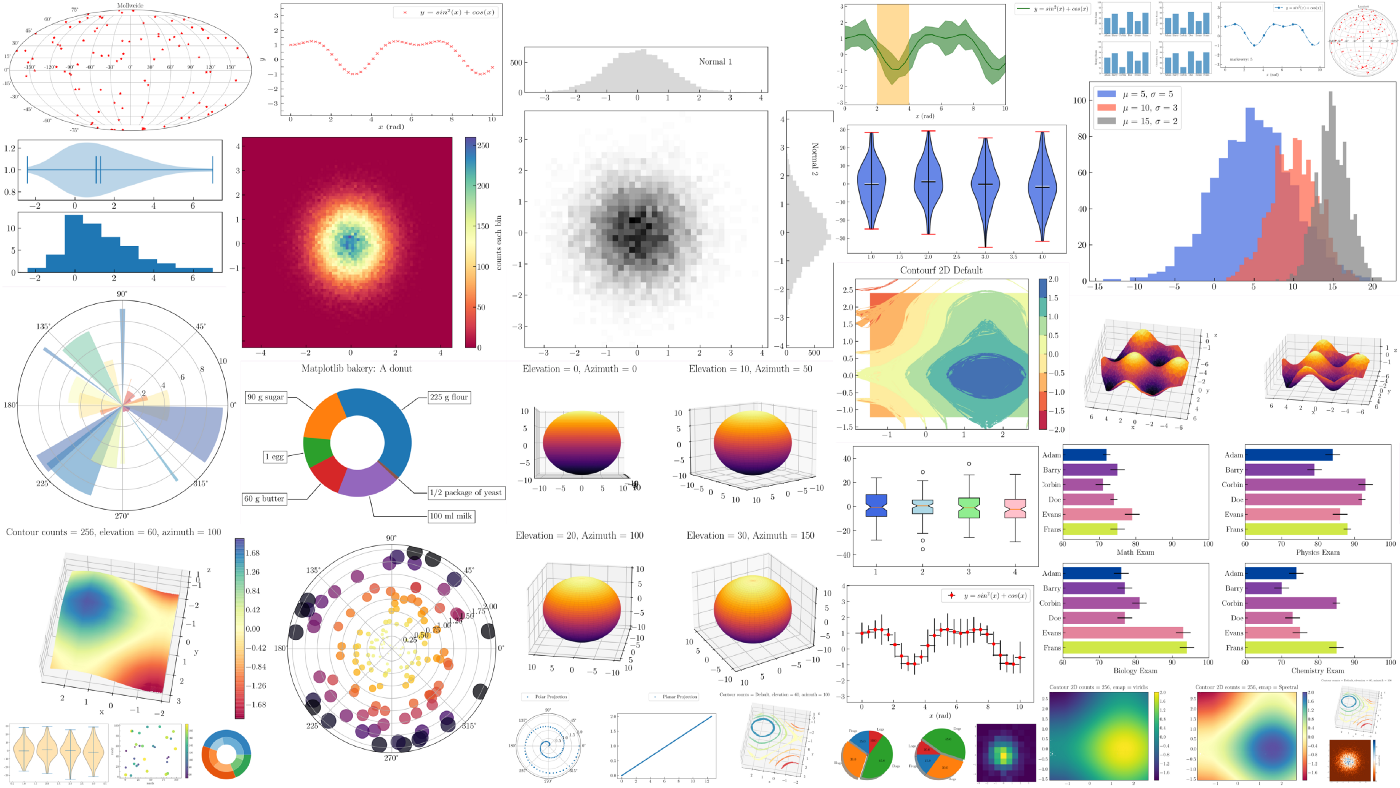
\includegraphics[width=10cm]{images/illustrations/viz_cheat_sheet.png}
   \end{figure}
\end{frame}

\begin{frame}\frametitle{Pourquoi ce cours}
   \begin{itemize}
      \item Formation accélérée : 1 journée, 7h \inlinegraphics{images/illustrations/run.jpeg}
      \item Objectifs
      \begin{itemize}
         \item Revoir et approfondir le choix du type de graphique
         \item Découvrir de nouvelles visualisations
         \item Découvrir comment les implémenter en python
         \item Comprendre les liens entre les différentes librairies Python
      \end{itemize}
   \end{itemize}
\end{frame}


% TODO compléter, reformuler
\begin{frame}\frametitle{Qu'est-ce que la \textit{data viz}}
   \begin{itemize}
      \item The graphical depiction of information and data is known as data visualisation. Data visualisation tools make it easy to view and comprehend trends, outliers, and patterns in data by utilising visual components like charts, graphs, and maps.
      \item It provides insights on one or more pages or screens to assist you keep track of events or activities at a glance. Unlike an infographic, which displays a static graphical representation, a dashboard displays real-time data by extracting complicated data points from massive data sets. 
      \item An interactive dashboard allows you to quickly sort, filter, and dive into many sorts of data. Data science approaches may be used to quickly understand what is occurring, why it is occurring, and what will occur next.
      \item Data visualization is the graphical representation of information and data. By using visual elements like charts, graphs, and maps, data visualization tools provide an accessible way to see and understand trends, outliers, and patterns in data. Additionally, it provides an excellent way for employees or business owners to present data to non-technical audiences without confusion.
      \item In the world of Big Data, data visualization tools and technologies are essential to analyze massive amounts of information and make data-driven decisions.
      \item Data visualization is a general term that describes any effort to help people understand the significance of data by placing it in a visual context. Patterns, trends and correlations that might go undetected in text-based data can be exposed and recognized easier with data visualization software. Data visualization is the presentation of quantitative information in a graphical form. In other words, data visualizations turn large and small data-sets into visuals that are easier for the human brain to understand and process. Data visualizations are surprisingly common in our everyday life, but they often appear in the form of well-known charts and graphs. It can be used to discover unknown facts and trends. Good data visualizations are created when communication, data science, and design collide. Data visualizations done right offer key insights into complicated data-sets in ways that are meaningful and intuitive. In this article, we would like to discuss about data visualization, importance of data visualization, data visualization tools etc.
   \end{itemize}
\end{frame}

% TODO add graphs to show
% TODO reformuler
\begin{frame}\frametitle{Dans quels domaines}
   \begin{itemize}
      \item Every STEM field benefits from understanding data—and so do fields in government, finance, marketing, history, consumer goods, service industries, education, sports, and so on. 
      \item Santé
      \item Business
      \item Finance
      \item Marketing
      \item etc.
   \end{itemize}
\end{frame}

% TODO reformuer
\begin{frame}\frametitle{Avantages}
   \begin{itemize}
      \item Making Big Data Digestible
      \item Greater Accessibility
      \item Greater Efficiency & Understanding
   \end{itemize}
\end{frame}

% TODO reformuer
\begin{frame}\frametitle{Risques}
   \begin{itemize}
      \item Something as simple as presenting data in graphic format may seem to have no downsides. But sometimes data can be misrepresented or misinterpreted when placed in the wrong style of data visualization. When choosing to create a data visualization, it’s best to keep both the advantages and disadvantages in mind. 
      \item Biased or inaccurate information.
      \item Correlation doesn't always mean causation.
      \item Core messages can get lost in translation.
   \end{itemize}
\end{frame}


% TODO: histoire de la data viz
% \begin{frame}\frametitle{Qu'est-ce que la \textit{data viz}}
%    \begin{itemize}
%       \item Origines
         % \item Source: \href{https://www.perceptualedge.com/articles/Whitepapers/Data_Visualization.pdf}{IBM Cognos Innovation Center}
%    \end{itemize}
% \end{frame}

% TODO: fusionner avec points du dessus
\begin{frame}\frametitle{Pourquoi faire de la \textit{data visualization}}
   \begin{itemize}
      \item Utiliser des graphiques plutôt qu'afficher un tableau de données permet:
      \begin{itemize}
         \item Une lecture plus rapide
         \item Une meilleure compréhension, plus intuitive
         \item D'être plus convainquant % (https://blog.reeport.io/fr/les-diagrammes-circulaires-ou-la-data-visualisation-pour-convaincre)
         \item D'aider à la prise de décision
      \end{itemize}
   \end{itemize}
\end{frame}

% TODO: ajouter chiffres
% \begin{frame}\frametitle{Pourquoi faire de la \textit{data visualization}}
%    \begin{itemize}
%       \item Enorme marché en constante évolution %(hors et y compris python - mais aussi outils BI classiques), évolution récente
%       \begin{itemize}
%           \item
%       \end{itemize}
%    \end{itemize}
% \end{frame}


% TODO: resume here (reprendre les points)
\begin{frame}\frametitle{Pourquoi faire de la \textit{data visualization}}  % quelles applications
   \begin{itemize}
      \item Dans quel cadre utiliser des visualisations de données ?
      \begin{itemize}
          \item Compréhension personnelle
          \item Rapports et présentations d'analyses et leurs résultats (équipe, direction)
      \end{itemize}
   \end{itemize}
\end{frame}

% TODO reformuler
\begin{frame}\frametitle{Pourquoi qui}
   \begin{itemize}
      \item Qui peut utiliser les visualisations de données
      \begin{itemize}
         \item développeurs
         \item analystes de données
         \item experts métier
         \item dirigeants
         \item tout le monde
      \end{itemize}
   \end{itemize}
\end{frame}

% TODO reformuler
\begin{frame}\frametitle{Comment faire de la data visualization, quels outils}
   \begin{itemize}
      \item (quel moyen: simples graphs sur Excel / en programmation, outils de dashboards Power BI / Tableau, outils intégrés à un progiciel)
   \end{itemize}
\end{frame}

% TODO REmplir
\begin{frame}\frametitle{Pourquoi avec Python, pour qui}
   \begin{itemize}
      \item 
   \end{itemize}
\end{frame}

% Reformuler
\begin{frame}\frametitle{Quels types de graphs?}
   \begin{itemize}
      \item différents types de données (séries temporelles - finance, audio, images 2D, 3D, graph networks, text avec word cloud). Chercher l'ensemble des types représentatbles avec des graphs
      \item examples pour les différents types de données (sans le code)
      \item exemples de graphs stylés
   \end{itemize}
\end{frame}


\end{document}
